%%%%%%%%%%%%%%%%%%%%%%%%%%%%%%%%%%%%%%%%%%%%%%%%%%%%%%%%%%%%%%%%%%%%%%%
%%%2345678901234567890123456789012345678901234567890123456789012345678901234567890
%%%        1         2         3         4         5         6         7         8

\documentclass[letterpaper, 10 pt, conference]{ieeeconf}  % Comment this line out if you need a4paper

%\documentclass[onecolumn, draftcls, journal]{IEEEtran}    %\newif\ifsinglecol


%\documentclass[a4paper, 10pt, conference]{ieeeconf}      % Use this line for a4 paper

\IEEEoverridecommandlockouts                              % This command is only needed if 
                                                          % you want to use the \thanks command

\overrideIEEEmargins                                      % Needed to meet printer requirements.

\usepackage[dvips]{graphicx}
\usepackage{ctable}
\usepackage{verbatim}
\usepackage{amsmath, amssymb}
\usepackage[dvips]{graphics}
\usepackage{algorithm}
%\usepackage{algorithmic}
\usepackage{bm}
\usepackage{graphics} % for pdf, bitmapped graphics files
\usepackage{epsfig} % for postscript graphics files
\usepackage{times} % assumes new font selection scheme installed
\usepackage{amsmath} % assumes amsmath package installed
\usepackage{amssymb}  % assumes amsmath package installed
%\usepackage{stfloats}
\usepackage{color}
\usepackage{lipsum}
%\usepackage{pmat} %<======= partition matrix 
\usepackage[T1]{fontenc} 
%\usepackage{algpseudocode}
\usepackage[noend]{algpseudocode}

\newcommand{\B}[1]{\mathbf{#1}}
\newcommand{\cb}[1]{\mathbf{#1}}
\newcommand{\bb}[1]{\textbf{#1}}
\newcommand{\bi}[1]{\boldsymbol{#1}}

%\def\BState{\State\hskip-\ALG@thistlm}

\newcommand\x{\times}
\newcommand\bigzero{\makebox(0,0){\text{\huge0}}}
\newcommand*{\bord}{\multicolumn{1}{c|}{}}

\pdfminorversion=4

\title{\LARGE \bf
Time Alignment of Trajectories Using Local Time Warping
}


\author{Guilherme Maeda$$% <-this % stops a space
\thanks{Intelligent Autonomous Systems Lab, Department of Computer Science,
		Technische Universit�t Darmstadt, Hochschulstr. 10, 64289 Darmstadt, Germany
        {\tt\small \{maeda\}@ias.tu-darmstadt.de}}%
}


\begin{document}

\maketitle
\thispagestyle{empty}
\pagestyle{empty}


%%%%%%%%%%%%%%%%%%%%%%%%%%%%%%%%%%%%%%%%%%%%%%%%%%%%%%%%%%%%%%%%%%%%%%%%%%%%%%%%
\begin{abstract}
This code does time alignment of trajectories by using local optimization.






\end{abstract}

%%%%%%%%%%%%%%%%%%%%%%%%%%%%%%%%%%%%%%%%%%%%%%%%%%%%%%%%%%%%%%%%%%%%%%%%%%%%%%%%
\section{Introduction}
\label{sec:intro}
 
Time alignment is usually achieved with Dynamic Time Warping (DTW) \cite{sakoe1978dynamic}.
As shown in Fig.~\ref{fig:dtw}, one issue is that of repeated indexes being attributed to different indexes of the other trajectory.
Although DTW provides the global optimal solution with respect to a distance cost, it does not take into account that trajectories generated by dynamical systems must be continuous. 
 
\begin{figure} 
	\centering
	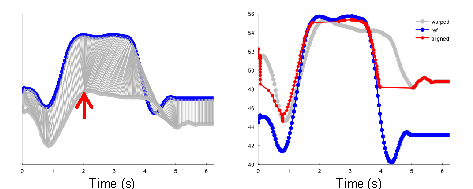
\includegraphics[scale=1.1, draft=false ]{./figures/dtw.pdf} %ok
	\caption{
		Vanilla implementation of dynamic time warping applied to very dissimilar trajectories.
		The plot at the left shows how the time indexes of the reference and warped trajectories relate to each other.
		Note that for a single index in one trajectory, multiple indexes of the other trajectory are allocated due to the minimum distance. One case is indicated by the arrow at time 2 seconds. The consequence of such repetitive correspondence is that the resulting aligned trajectory may present discontinuities (right).
	}
	\label{fig:dtw}
\end{figure}
 
As shown in Fig.~\ref{fig:dtwss}(a) shows the mapping between the time indexes of two trajectories.
At the location indicated by the arrow, the vertical segment indicates the issue of discontinuity, which leads to unnatural alignment.
This issue is usually solved with a slope constraint heuristic.
In this paper we propose solving this issue by forcing a continuous and smooth warping function as shown in Fig.~\ref{fig:dtwss}(b).
This approach generates a one-to-one association of the time indexes which is naturally fit for local optimization of the function $f(\bi \theta)$.

\begin{figure} 
	\centering
	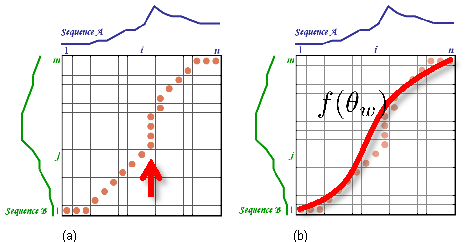
\includegraphics[scale=1.1, draft=false ]{./figures/dtwss.pdf} %ok
	\caption{
	(a) Index mapping with DTW \cite{dtw_webpage}. The part indicated by the arrow causes discontinuities in the trajectory, which is unnatural for physical dynamical systems.
	(b) We propose solving the slope problem by using a warping function that is continuous and smooth by construction. The algorithm forces a one-to-one association of indexes which is more suitable for dynamical systems.
	}
	\label{fig:dtwss}
\end{figure}



%\section{Related Work} 
%\label{sec:related_work}
%\lipsum[1-5] 


\section{The Algorithm}
%Proposed Method}
\label{sec:proposed_method}

Consider the mapping $F: t^{r}_{1:T} \mapsto t^{w}_{1:T}$ that maps the time indexes of a reference 
trajectory with associated time vector $t^{r}_{1:T}$ to a query trajectory whose associated time vector $t^{w}_{1:T}$ is to be found.
Note that one of the trajectories must be resampled such that both query and reference trajectories have the same number of time steps $T$.
The algorithm does not modify the number of time steps, but the duration between each time step.
Define the cumulative cost based on DTW as 
\begin{equation}
	C = \sum_{t=1}^T \| \bi x^r( t^{r}_t) - \bi x^q( t^w_t )    \|,
	\label{eq:dtwcost}
\end{equation}
where $\bi x^r$ is the reference trajectory for time alignment, and $\bi x^q$ is the query trajectory to be aligned.

The goal of the method is to find a warping mapping function $F$ such that the cumulative cost is minimized.
We initially parameterize the warping function with parameters $\bi \theta = \{\theta_0, \ \bi \theta_w\}$ such that
%\begin{equation}
%	\begin{split}
%		t^w_{1:T} & = \theta_0 + f(\bi \theta_w)  t^{r}_{1:T}\\
%	        	  & = \theta_0 + \Psi \theta_w  t^{r}_{1:T}
%	\end{split}	
%\end{equation}
\begin{equation}
	\bi s_{1:T}  = f(\bi \theta_w),
	\label{eq:ss}
\end{equation}
and 
\begin{equation}
	\bi t^w_{1:T}  = \theta_0 + \bi s \odot \bi t^{r}_{1:T}.
	\label{eq:ww}
\end{equation}
The function $f(\bi \theta_w)$ is the local warping function, previously illustrated in Fig.~\ref{fig:dtwss}(b) and returns a vector of scaling values for each time step of the original reference time.
In \eqref{eq:ww}, the  second term is the element wise product of $\bi s_{1:T}$ and the reference time  $\bi t^r_{1:T}$.

The scalar parameter $\theta_0$ changes the start instant of $t^w_{1:T}$.
This is useful when both reference and query trajectories are identically in shape, but start at different times.
%
%The second term is the product of a diagonal warping matrix $\bi W \in \mathbb{R}^{T \times T}$ and the reference time  $\bi t^r_{1:T} \in \mathbb{R}^T$.
%
In the particular case when the reference and query trajectories are already aligned, $\theta_0=0$ and \eqref{eq:ss} returns a vector of ones.
This is usually the standard initial guess of parameters to initialize the optimization.

To enforce that $f(\bi \theta_w)$ is a smooth function, we use the parameterization
\begin{equation}
	\bi s_t = \sum_{n=1}^N  \bi (\Phi_t)_n \bi (\theta_w)_n.
	\label{eq:st}
\end{equation}
where $(\Phi_t)_n$ is the value of the n-th radial basis function at time $t$. 
The dimension of $\bi \theta_w \in \mathbb{R}^{N}$ is the defined by the number of $N$ basis functions to be used.


The method consists in using a local optimization method, such as gradient descent, to update $\bi \theta = \{\theta_0, \ \bi \theta_w\}$ such that the cost 	\eqref{eq:dtwcost} is minimized.
In the current implementation, gradient descent with Jacobian computed by finite differences is used.
The source code with an example can be found in


%The pseudo-code is provided in 
%
%\begin{algorithm}
%	\caption{Local Time Warping}\label{ltw}
%	\begin{algorithmic}[1]
%		\For{ $k < nMax$ or Converged }
%		\State $\bi \theta_{k}  \gets \bi \theta_{k-1} + \alpha \bi J^{-1} C$
%		\State $\bi t^w_{1:T} \gets \text{NewTimeWarping}(  \theta_0, \  \bi s_{1:T}, \ \bi t^{r}_{1:T}) $
%		\State $C \gets \text{ComputeCumulativeCost}( \bi x^q( t^w_t ),\  \bi x^r( t^r_t )  ) $.		
%		%		\State $i \gets i+\max(\textit{delta}_1(\textit{string}(i)),\textit{delta}_2(j))$.
%		%		\EndProcedure
%		\EndFor
%	\end{algorithmic}
%\end{algorithm}
%
%\begin{algorithm}
%	\caption{Local Time Warping}\label{euclid}
%	\begin{algorithmic}[1]
%%		\State $\textit{stringlen} \gets \text{length of }\textit{string}$%
%%		\State $i \gets \textit{patlen}$
%%		\If {$i > \textit{stringlen}$} \Return false
%%		\EndIf
%%		\State $ \gets \textit{patlen}$
%%		\If {$\textit{string}(i) = \textit{path}(j)$}
%%		\State $j \gets j-1$.
%		\For{ $k < nMax$ or Converged }
%		\State $\bi s_{1:T}  \gets  f(\bi \theta_w)$ //compute scaling vector with \eqref{eq:st}
%		\State $\bi t^w_{1:T} \gets \text{NewTimeWarping}(  \theta_0, \  \bi s_{1:T}, \ \bi t^{r}_{1:T}) $
%		\State $C \gets \text{ComputeCumulativeCost}( \bi x^q( t^w_t ),\  \bi x^r( t^r_t )  ) $.		
%%		\State $i \gets i+\max(\textit{delta}_1(\textit{string}(i)),\textit{delta}_2(j))$.
%%		\EndProcedure
%		\EndFor
%	\end{algorithmic}
%\end{algorithm}





\section{Experiments}
\label{sec:experiments}



%
%\section{Conclusions}
%\label{sec:conclusions}
%
\lipsum[1-2] 



\section{Acknowledgments}

%
%The research leading to these results has received funding from the TU Darmstadt, from the European Community's Seventh Framework Programme (FP7-ICT-2013-10) under grant agreement 610878 (3rdHand).
%
%%The research leading to these results has received funding from the European Community's Seventh Framework Programmes (FP7-ICT-2013-10) under grant agreement 610878 (3rdHand) and (FP7-ICT-2009-6) under grant agreement 270327 (ComPLACS).

%\bibliographystyle{IEEEtran}
\bibliographystyle{ieeetran}
%\bibliography{bibliography_database}

\IfFileExists{C:/Users/mito/Dropbox/Papers/pdf/gjmRef.bib}{\bibliography{C:/Users/mito/Dropbox/Papers/pdf/gjmRef}}{}
%\IfFileExists{C:/Windows/notepad.exe}{\bibliography{C:/gjm/Dropbox/Papers/pdf/gjmRef}}{}
\IfFileExists{/home/v5i7/Documents/v5i7.txt}{\bibliography{/home/v5i7/Dropbox/Papers/pdf/gjmRef}}{}
\IfFileExists{/home/maeda/Documents/hahn.txt}{\bibliography{/home/maeda/Dropbox/Papers/pdf/gjmRef}}{}

\end{document}
